\chapter{Meet the Billionaire Who Created LinkedIn (Then Sold It for \$26B)}

This lecture opens by showing us the answer before it shows us the method. We are given the \$26 billion sale, the later scale of LinkedIn's revenue, the two-thirds of smart friends who thought the venture would fail, the brutality of venture-capital selection, and the now-famous ability to recognize an exceptional company almost immediately. Only then does the conversation rewind and ask the real question: what kind of strategic reasoning makes such outcomes possible? There are no validated mathematical screenshots for this lecture, so the equations and diagrams below are cautious transcript-derived reconstructions. The mathematics is therefore not blackboard mathematics. It is the mathematics of filters, thresholds, repeated play, network growth, and compounding over long horizons.

\section{Cold Open: Outcome, Doubt, and Filter Math}

The lecture begins in teaser form. Before we are told what to think, we are shown what is at stake. LinkedIn is introduced through its sale to Microsoft, through the later magnitude of the business, and through the fact that a large majority of informed observers initially expected failure. This sequence matters. The lecture wants us to feel the asymmetry first, and only afterward to ask how such asymmetry is produced.

We can collect the opening numerical anchors as follows:
\begin{align}
V_{\mathrm{LI,sale}} &= \$26\,\mathrm{B}, &
R_{\mathrm{LI,last}} &\approx \$16\,\mathrm{B/yr}, \\
V_{\mathrm{PayPal,sale}} &\approx \$1.5\,\mathrm{B}, &
K_1 &\approx \$5\,\mathrm{M}, \\
K_{\mathrm{tot}} &\approx \$140\,\mathrm{M}, &
d &> \frac{2}{3}.
\end{align}
Here \(d\) denotes the fraction of Hoffman's smart friends who thought LinkedIn would be a complete failure. It is worth separating these numbers with some care. The sale price of LinkedIn is not the same quantity as Hoffman's personal yearly income, and the later annual revenue of LinkedIn is not the same quantity as its sale value. The interview moves quickly across these scales because it is staging the magnitude of the story. Our notes should keep the scales distinct.

The other numerical fact in the cold open is the venture-capital funnel:
\begin{equation}
N_{\mathrm{deals}} \in [600,800], \qquad N_{\mathrm{yes}} \in [0,2].
\end{equation}
This is already enough to tell us that the founder does not enter an open agora of ideas. He enters a severe compression chamber.

\paragraph{Worked example: the venture filter.}
If we use Hoffman's own bounds, then the implied acceptance rate satisfies
\begin{equation}
p_{\mathrm{yes}}=\frac{N_{\mathrm{yes}}}{N_{\mathrm{deals}}}\lesssim \frac{2}{600}\approx 3.3\times 10^{-3}.
\end{equation}
So the optimistic upper bound is below one third of one percent. If the numerator is \(0\), the rate is \(0\). The exact fraction is not the point. The point is that ordinary plausibility does not survive such a filter. One must bring either extraordinary evidence or a live contrarian thesis.

\begin{figure}
\begin{center}
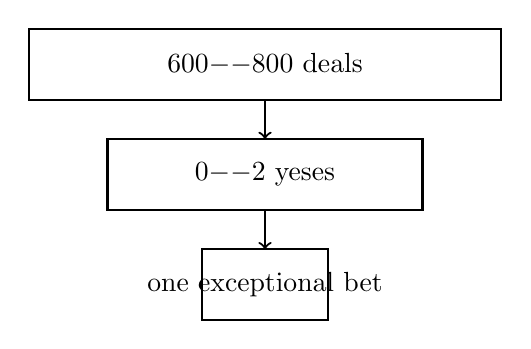
\begin{tikzpicture}
\draw[thick] (0,0) rectangle (6,0.9);
\draw[thick] (1.0,-1.4) rectangle (5.0,-0.5);
\draw[thick] (2.2,-2.8) rectangle (3.8,-1.9);
\draw[->,thick] (3,0) -- (3,-0.5);
\draw[->,thick] (3,-1.4) -- (3,-1.9);
\node at (3,0.45) {$600\text{--}800$ deals};
\node at (3,-0.95) {$0\text{--}2$ yeses};
\node at (3,-2.35) {one exceptional bet};
\end{tikzpicture}

{\small Transcript-derived venture filter: hundreds of yearly opportunities contract to almost nothing.}
\end{center}
\end{figure}

Two further signals are planted here and only explained later. First, Hoffman says that when he met the Airbnb founders, he knew within two minutes that he wanted to invest. Second, when the host asks how one might make a billion dollars in a year, Hoffman will later resist the frame and redirect us to a ten-year game. Thus even the teaser already contains the lecture's deep grammar: harsh selection, rare surprise, and long horizon.

\section{Burn the Boats Early, but Preserve the Right to Play Again}

After the host's arrival, greeting, and a brief transcript splice through an AI aside, the conversation stabilizes and returns to the early LinkedIn years. This is an important reset. The lecture stops being a montage of outcomes and becomes a sequence of causal questions. What was the moment at which Hoffman knew he was going all in?

His answer is sharper than the usual entrepreneurial folklore. We do not first achieve confidence and only then commit. We commit early. We accept that the move may fail. What matters is that the failure not destroy the ability to make another move. In that sense, the first doctrine of the lecture is not heroic confidence. It is disciplined replay.

A compact reconstruction is
\begin{equation}
U_{\mathrm{win}} \gg L_{\mathrm{fail}}, \qquad L_{\mathrm{fail}} < L_{\mathrm{ruin}}.
\end{equation}
The first inequality captures asymmetry: if the bet works, it works big. The second captures survivability: if it fails, the founder is not strategically dead.

\begin{definition}
A repeatable entrepreneurial risk is a risk with disproportionately large upside, real but tolerable downside, and a failure mode that does not eliminate future participation in the game.
\end{definition}

Let us be careful here. ``Burn the boats'' does not mean reckless theater. It means that hesitation cannot be the governing principle in a field where visible safety usually arrives after the edge has vanished. The lecture wants us to see commitment and survivability at the same time.

\subsection{Question \& Answer}

\paragraph{Question.}
Why commit before we feel certain?

\paragraph{Answer.}
Because certainty comes too late. If a path is already obviously safe, then the unusual upside has probably already been arbitraged away. Hoffman's point is not that fear disappears; he says explicitly that everyone is somewhat afraid of failure. The point is that fear need not be terminal. We arrange the bet so that failure teaches, stings, and perhaps delays us, but does not remove us from the field.

This is why the lecture repeatedly returns to the phrase ``play again.'' The founder's problem is not to enter a world without uncertainty. The founder's problem is to enter uncertainty on terms that preserve another move.

\section{Choosing the Right Game and the Right Geography}

The host then asks the natural follow-up: where did the confidence come from? Hoffman answers by shifting the discussion away from generic self-belief and toward strategic placement. He knew what game he was playing, and he knew the geography in which that game had the best chance to compound.

A simple notation is useful here:
\begin{equation}
g(\mathrm{Silicon\ Valley})=\mathrm{software}, \qquad
g(\mathrm{New\ York})=\mathrm{finance}, \qquad
g(\mathrm{Los\ Angeles})=\mathrm{media}.
\end{equation}
This is not a universal law. It is a strategic map. The lecture's point is that games cluster. If we choose the right domain but the wrong arena, we are not necessarily out of the game, but we are likely to be playing uphill.

The earlier notion of replay now becomes more precise. If the arena itself supports multiple attempts, then a single failed move does not exile us from the whole field. Silicon Valley, as Hoffman describes it, is not merely a place for software success. It is a place where software attempts can be repeated, revised, and recombined.

At this point the lecture is ready for a more delicate question. Even if software in Silicon Valley was the right game, why did LinkedIn itself look so dubious? What was the specific objection that had to be answered?

\section{The Network Bootstrap Problem at LinkedIn}

Now we arrive at the local conceptual knot around which much of the chapter turns. In 2003, Hoffman says, many people in Silicon Valley thought the consumer internet was finished. Amazon, Google, and PayPal already existed, but the next wave of social products did not yet command confidence. LinkedIn, in particular, seemed to many people like an awkward variant of a category that itself had not been justified.

The objection is extremely clean. A network is least convincing precisely when it is smallest. The first person in gets almost no value. The next few users may already know one another, so again the immediate value seems negligible. If this is the case, why should anyone continue joining?

A cautious reconstruction is
\begin{equation}
V_{\mathrm{net}}(n)\approx 0 \qquad \text{for very small } n,
\end{equation}
together with the qualitative claim that once the network thickens enough, the marginal value turns decisively positive:
\begin{equation}
V'_{\mathrm{net}}(n) > 0 \qquad \text{after the network reaches a viable thickness.}
\end{equation}
The transcript does not give us an explicit formula for \(V_{\mathrm{net}}(n)\), and we should not pretend otherwise. What it does give us is the shape: a discouraging flat region at the beginning, followed by a regime in which each additional participant makes the whole network more useful.

\begin{figure}
\begin{center}
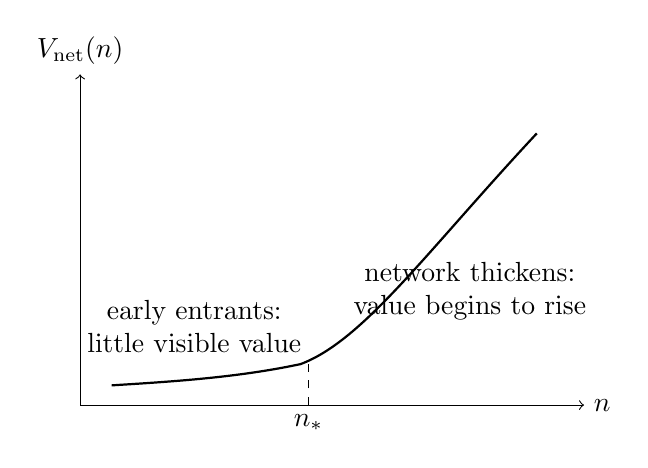
\begin{tikzpicture}[scale=1.0]
\draw[->] (0,0) -- (6.4,0) node[right] {$n$};
\draw[->] (0,0) -- (0,4.2) node[above] {$V_{\mathrm{net}}(n)$};
\draw[thick] (0.4,0.25) .. controls (1.2,0.30) and (2.0,0.35) .. (2.8,0.52)
             .. controls (3.6,0.82) and (4.4,1.95) .. (5.8,3.45);
\draw[dashed] (2.9,0) -- (2.9,0.60);
\node[below] at (2.9,0) {$n_\ast$};
\node[align=center] at (1.45,1.0) {early entrants:\\little visible value};
\node[align=center] at (4.95,1.45) {network thickens:\\value begins to rise};
\end{tikzpicture}

{\small Transcript-derived sketch of the LinkedIn bootstrap problem: the early regime looks empty, and only later does network value begin to reveal itself.}
\end{center}
\end{figure}

\subsection{Question \& Answer}

\paragraph{Question.}
How can a network with no initial value still become valuable?

\paragraph{Answer.}
Not because the first users are secretly extracting large value, but because the founder may have a credible path by which the network reaches the regime where value begins to reinforce growth. The lecture's key phrase is really the contrarian one: what do I know that they do not know? In this case, the answer is not mystical. It is structural. Hoffman believed he could get the network to grow before users felt substantial value inside the system.

\paragraph{Bootstrap derivation.}
We can write the logic in steps:
\begin{enumerate}
\item For \(n\) very small, \(V_{\mathrm{net}}(n)\) is nearly flat.
\item This generates the skeptical verdict: no immediate value, therefore no growth.
\item The founder supplies a thesis \(\theta\): there exists a workable path from small \(n\) to a threshold \(n_\ast\).
\item Once \(n\geq n_\ast\), each additional participant improves the usefulness of the system, so growth and value begin to reinforce one another.
\end{enumerate}

This is the strongest local tension in the lecture, and it should remain visible in the notes. The late business lesson that monetization can come after network growth is powerful only because this earlier puzzle has first been stated honestly.

\section{From Product-Maker Identity to Visible Scale}

After the network problem, the lecture steps outward into biography. Hoffman says he did not come from a family of entrepreneurs but from a family of civil servants. His grandfather apparently viewed industrial ambition with a certain discomfort. This matters because the entrepreneurial turn is presented not as inheritance but as selection.

The turning point, as the interview gives it, runs through Stanford, artificial intelligence, and then a more definite decision: the desire to create new products. Apple and Fujitsu appear here not as destinations but as intermediate stations. The decisive point is that Hoffman wanted to make new things, not merely occupy a role inside existing organizations.

Then the interview loops back to public scale. The host again asks about money, and the lecture again supplies the concrete numbers: LinkedIn later produced roughly \$16 billion in yearly revenue, and LinkedIn was sold to Microsoft for \$26 billion. Satya Nadella and Bill Gates come to LinkedIn's office and express interest. This matters because the lecture is preparing the next question. Visible success is not the end of the discussion. It is the bridge to credibility. How does one build relations with people of that level before the success has already occurred?

\section{Credibility, Networking, and the Give-Before-Ask Rule}

After a long promotional interruption, the interview returns with one of its cleanest doctrines. The question is now about networking, but Hoffman's answer is really a theory of value exchange. The first move is not to ask for help. The first move is to ask what we can offer.

A cautious update rule is
\begin{equation}
C_{t+1}=C_t+\Delta C(U_t),
\end{equation}
where \(C_t\) is relationship capital at time \(t\), and \(U_t\) is the usefulness of what we bring. The transcript does not imply that every attempt at usefulness succeeds. It implies something subtler: usefulness is the correct state variable, while extractive asking is generally the wrong one.

We may sharpen the point as a sign rule:
\begin{equation}
U_t>0 \Longrightarrow \Delta C(U_t)>0,
\qquad
U_t=0 \text{ with ask-first behavior } \Longrightarrow \Delta C(U_t)\leq 0.
\end{equation}
Again, the notation is only schematic. But it matches the lecture. Satya Nadella calls Hoffman because Hoffman can explain Silicon Valley. Bill Gates is not approached through praise, but through information: here is something happening in technology, perhaps in AI, that may be useful to you.

\subsection{Question \& Answer}

\paragraph{Question.}
How do we build relationships with A players before we have much credibility?

\paragraph{Answer.}
Not by mimicking status, and not by confusing symbolic contact with real connection. The lecture insists on a stronger criterion. A relation begins when we offer a pattern, an observation, an introduction, or a judgment that actually helps the other person. Credibility is then not a precondition entirely separate from value. It is built through value.

Hoffman then classifies successful people by three recurring traits:
\begin{itemize}
\item curiosity, the intense desire to learn;
\item grit, the refusal to stop at the first obstruction;
\item contrarian understanding, the ability to see something that others do not yet see.
\end{itemize}
The third term returns us directly to LinkedIn and to Airbnb. The lecture is telling us that networking and investment are not separate from thought. To be useful to strong people, one must have seen something worth bringing.

This also explains Hoffman's impatience with much of ordinary networking. ``Here is my card'' is not a relation. The real thing is a connection in which two sides are, in fact, helping one another.

\section{Negotiation, Decisions, and the Multi-Time Game}

The interview then moves into a final large synthesis, but it is better to hear it as a sequence of local steps. First comes negotiation. Then advice. Then failure. Only after that does the lecture broaden into fundraising, scaling, and long-horizon compounding.

\subsection{Negotiation as buyer pull}

Hoffman's line is memorable because it compresses a whole psychology into a few words: companies are bought, not sold. What matters is not merely the object itself but the posture under which the object is encountered. If we arrive trying to sell, we grant the other side a superior stance. If they come to want the thing, the geometry changes.

A minimal schematic is
\begin{equation}
D_{\mathrm{buy}}\uparrow \Longrightarrow P_{\mathrm{deal}}\uparrow,
\end{equation}
where \(D_{\mathrm{buy}}\) denotes buyer desire and \(P_{\mathrm{deal}}\) denotes the feasibility of closing the deal. The equation is not a bargaining model. It is a transcript-faithful summary of the psychology Hoffman describes. The aim is to increase buyer pull rather than visible seller push.

The lecture's own example is LinkedIn and Microsoft. Hoffman does not narrate an outbound liquidation. He narrates interest arriving from Satya Nadella and Bill Gates. That is exactly the form he later recommends.

\subsection{Question \& Answer}

\paragraph{Question.}
Why does ``bought, not sold'' matter so much?

\paragraph{Answer.}
Because the other side's sense of agency changes the deal. If they feel they are being sold to, they step back, protect status, and judge from above. If they feel they have discovered something they want, they lean in. The lecture is really about the psychology of initiative: the strongest transactions often succeed when acquisition feels like the buyer's own idea.

\subsection{Door \(A\), door \(B\), and repeated play}

From negotiation the lecture pivots into advice from Hoffman's father. Making a decision is hard because it reduces short-term possibility. If we choose door \(A\), we no longer choose door \(B\). Yet this reduction is not merely a loss. It is the only way long-run opportunity acquires form.

We may summarize the rule by
\begin{equation}
O_{\mathrm{short}}\downarrow, \qquad O_{\mathrm{long}}\uparrow.
\end{equation}
Without local closure, long-run structure never appears.

The same logic governs Hoffman's account of SocialNet. It did not pay off in the immediate financial sense. But it got him into the journey. This is not an attempt to rename failure as success. It is an insistence that failure belongs inside a repeated sequence:
\begin{equation}
X_{t+1}=F(X_t,\ell_t),
\end{equation}
where \(\ell_t\) denotes the learning extracted from step \(t\). The mathematical point is simple. The output of a failed venture need not be the zero state. It may be the state from which a later and stronger move becomes possible.

\begin{figure}
\begin{center}
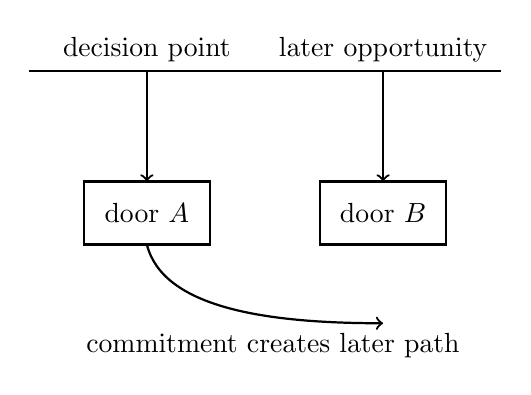
\begin{tikzpicture}[scale=1.0]
\draw[thick] (0,0) -- (6,0);
\draw[->,thick] (1.5,0) -- (1.5,-1.4);
\draw[->,thick] (4.5,0) -- (4.5,-1.4);
\node[above] at (1.5,0) {decision point};
\node[above] at (4.5,0) {later opportunity};

\draw[thick] (0.7,-1.4) rectangle (2.3,-2.2);
\draw[thick] (3.7,-1.4) rectangle (5.3,-2.2);

\node at (1.5,-1.8) {door \(A\)};
\node at (4.5,-1.8) {door \(B\)};

\draw[->,thick] (1.5,-2.2) .. controls (1.7,-3.0) and (3.0,-3.2) .. (4.5,-3.2);
\node[below] at (3.1,-3.2) {commitment creates later path};
\end{tikzpicture}

{\small Transcript-derived decision sketch: choosing one door narrows the short run, but only commitment generates a long run worth having.}
\end{center}
\end{figure}

\section{Capital, Blitzscaling, and the Ten-Year Game}

Now the lecture broadens for the last time. A lawyer once told Hoffman that he was not yet in a position to raise money and that he needed first to prove product credentials. This is painful advice, but in the structure of the lecture it is exemplary advice. It replaces fantasy capital with earned legibility.

When LinkedIn raises money, the amounts are concrete:
\begin{equation}
K_1 \approx \$5\,\mathrm{M}, \qquad K_{\mathrm{tot}} \approx \$140\,\mathrm{M}.
\end{equation}
By this stage, the founder is not merely pitching a clever idea. He is presenting evidence, judgment, and positioning. Investors, the lecture says, are looking for something that could be very large, something aligned with an identifiable wave, and some reason to believe that \emph{this} founder should receive the bet. That is why the venture filter from the opening returns here with sharper force.

The Airbnb anecdote now lands with more precision. The lecture's point is not simply that Hoffman is quick. It is that exceptional founders often present a thesis that is legible precisely because it is surprising. They appear to have seen something no one else has seen.

From there the argument widens into industries. Bits, Hoffman says, will accelerate atoms. AI will speed drug discovery, robotics, manufacturing, and even homebuilding. The transcript is forward-looking here, but the logical structure does not change. A good venture thesis connects an initially invisible mechanism to a future reorganization of the physical world.

The lecture then turns to blitzscaling. Here the advice is operational rather than metaphysical. If we are truly scaling fast, we cannot keep taking our foot off the accelerator every time a new market, product, or hire appears. We must learn to decide in motion.

The companion hiring advice is equally structural. Hoffman describes himself as a creative problem solver. Therefore he needs partners who are operationally rigorous and keep the trains running on time. Scale is not the enlargement of a lone founder. It is the formation of a complementary system.

Now the conversation reaches one of its most instructive late reversals. Hoffman says he initially expected individual subscriptions to be LinkedIn's primary business. But companies began approaching LinkedIn and asking to buy. The team described the product in a deck, sent it out, and got purchase orders back. The market, in effect, revealed the monetization layer.

This late lesson can be written schematically as
\begin{equation}
N(t)\uparrow \quad \text{first}, \qquad M=M(N) \quad \text{later}.
\end{equation}
First the network grows. Then monetization crystallizes on top of the network. This is why the earlier network puzzle mattered so much. The lecture ends by resolving it. Once the network exists at the right scale, monetization need not be forced too early.

The final horizon question makes the same point in temporal form. Hoffman says he almost never plays a one-year game. He plays a ten-year game. A cautious reconstruction is
\begin{equation}
X_{10}=X_0(1+g)^{10}.
\end{equation}
No numerical \(g\) is provided, and none should be invented. The formula is there only to represent the lecture's qualitative point: most people think too locally, and the difference between a one-year and a ten-year horizon is not additive but compounding.

We may summarize the contrast very simply:
\begin{equation}
H_{\mathrm{short}}=1, \qquad H_{\mathrm{long}}=10.
\end{equation}
The lecture is telling us that horizon is itself a source of edge. Most people do not think about what compounds when it is given enough time.

Hoffman also says he was probably around \(38\) when he became a billionaire, though he marks that recollection as approximate. Even this detail fits the larger structure. The public milestone arrives long after the internal logic is already in motion.

\section{Summary}

The lecture begins with spectacle and then patiently asks what hidden machinery could produce it. The answer is not a single trick. It is a chain of linked strategic principles. We commit before certainty is available, but we arrange the risk so that failure does not end the game. We choose the right game and the right geography. We understand that a network may look empty before it crosses the threshold at which value becomes self-reinforcing. We build relationships by offering value before asking for anything in return. We negotiate by increasing buyer desire rather than seller pressure. We understand that commitment narrows the short run in order to open the long run. We raise capital only after becoming legible enough to deserve it. We scale by deciding in motion. We let monetization come after network growth. And we think in decades rather than in seasons.

The final sentence of the lecture gathers all of this into human form. Life, Hoffman says, is a team sport, not an individual sport. Pick your team. This is not a sentimental flourish. It is the final theorem of the chapter. LinkedIn is a network business; PayPal is described as a network; networking itself is only real when it becomes mutual help; negotiation depends on the psychology of the other side; compounding requires that we stay alive in the game; and large-scale execution requires complementary partners. The mathematics here is therefore the mathematics of connectedness: filters, thresholds, update rules, and repeated play, all unfolding over enough time for the invisible curve to bend upward.